%% It is just an empty TeX file.
%% Write your code here.
% !TEX encoding = UTF-8 Unicode
\documentclass[a4paper, 12pt]{article}   	% use "amsart" instead of "article" for AMSLaTeX format
\usepackage[left=20mm, top=15mm, right=10mm, bottom=15mm]{geometry}    

            
\usepackage[parfill]{parskip}    		% Activate to begin paragraphs with an empty line rather than an indent
\usepackage{graphicx}				% Use pdf, png, jpg, or eps§ with pdflatex; use eps in DVI mode
\usepackage[14pt]{extsizes}
\usepackage{setspace,amsmath}
\usepackage{mathtools}
\usepackage{ dsfont }
\usepackage{amsmath,amssymb}
\usepackage[unicode]{hyperref}

\usepackage{xcolor}
\usepackage{color}
\usepackage{minted}
\usepackage{caption}

\usepackage{array}
\newcolumntype{P}[1]{>{\centering\arraybackslash}p{#1}}

\usepackage{cmap} % Улучшенный поиск русских слов в полученном pdf-файле
\usepackage[T2A]{fontenc} % Поддержка русских букв
\usepackage[utf8]{inputenc} % Кодировка utf8
\usepackage[english, russian]{babel} % Языки: русский, английский

								% TeX will automatically convert eps --> pdf in pdflatex		
\usepackage{amssymb}

\begin{document}
\begin{titlepage}

\thispagestyle{empty}

\begin{center}
Федеральное государственное бюджетное образовательное учреждение высшего профессионального образования Московский государственный технический университет имени Н.Э. Баумана
\end{center}


\vfill

\centerline{\large{Лабораторная работа №5. Вариант 1.}}

\centerline{\large{«Методы поиска условного экстремума»}} 

\centerline{\large{по курсу}}
\centerline{\large{«Методы оптимизации»}}


\vfill

Студент группы ИУ9-82 \hfill Белогуров А.А.

Преподаватель \hfill Каганов Ю.T. 
\vfill

\centerline{Москва, 2018}
\clearpage
\end{titlepage}

\newpage
\setcounter{page}{2}

\tableofcontents

\newpage

\section{Цель работы}

\begin{enumerate}
    \item Изучение алгоритмов условной оптимизации.
    \item Разработка программ реализации алгоритмов условной оптимизации.
    \item Нахождение оптимальных условий решений для задач с учетом ограничений.
\end{enumerate}

\newpage

\section{Постановка задачи}
    \textbf {Дано}: 1 Вариант. Функция Розенброка на множестве $R^2$:
    \begin{equation}
        f(x) = \sum^{n-1}_{i=1}{[a(x_i^2 - x_{i+1})^2 + b(x_i - 1)^2] + f_0},
    \end{equation}
    
    где 
    \begin{equation}
        a = 50, \quad b = 2, \quad f_0 = 10, \quad n = 2,
    \end{equation}
    
    тогда функция $f(x)$ будет выглядеть следующим образом:
    \begin{equation}
        f(x) = 50 * (x_0^2 - x_1)^2 + 2 * (x_0 - 1)^2 + 10
    \end{equation}
    
    Функции ограничений:
    \begin{equation}
        \begin{cases}
            g_1(x_1, x_2) = x_1^2+x_2^2 - 1 \leq 0 \\
            g_2(x_1, x_2) = -x_1 \leq 0 \\
            g_3(x_1, x_2) = -x_2 \leq 0
        \end{cases}
    \end{equation}
    

    \begin{enumerate}
        \item Найти условный экстремум методами:
        \begin{enumerate}
            \item Штрафных функций;
            \item Барьерных функций;
            \item Модифицированных функций Лагранжа;
            \item Проекции градиента.
        \end{enumerate}
        \item Найти все стационарные точни и значения функций, соотвестсвующие этим точкам. 
        \item Оценить скорость сходимости указанных алгоритмов.
        \item Реализовать алгоритмы с помощью языка программирования высокого уровня.
    \end{enumerate}
    

\newpage
\section{Исследование}
    Найдем глобальные экстремумы функции 
    \begin{equation}
         f(x) = 50(x_0^2 - x_1)^2 + 2(x_0 - 1)^2 + 10
    \end{equation}
    с помощью сервиса WolframAlpha.com:
    
     \begin{equation}
        min(f(x)) = 10,\quad (x_0, x_1) = (1, 1)
    \end{equation}
    
    \begin{center}
        \begin{minipage}{0.7\linewidth}
            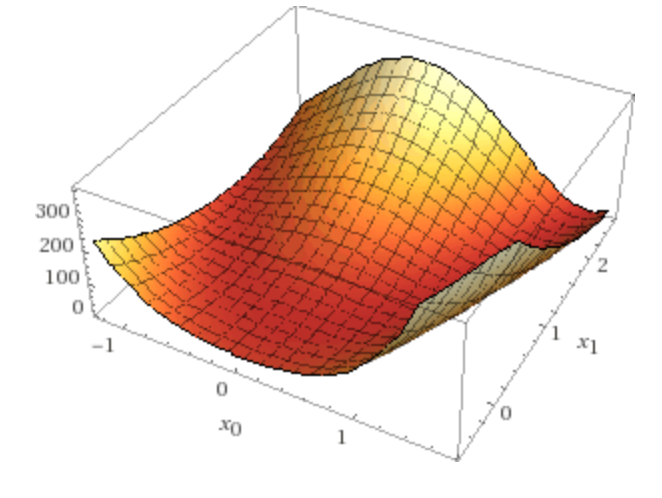
\includegraphics[width=\linewidth]{img/function}
            \captionof{figure}{График функции $f(x)$}
        \end{minipage}
    \end{center}
    
\subsection{Метод щтрафных функций.}
    Идея метода заключается в сведении задачи на условный минимум к решению последовательности задач поиска безусловного минимума вспомогательной функции: 
    \begin{equation}
        F(x, r^k) = f(x) + P(x, r^k) \rightarrow \min_{x \in R^n},
    \end{equation}

    где $P(x, r^k)$ -  штрафная функция, $r^k$ - параметр штрафа, задаваемый на каждой k- й итерации. Это связано с возможностью применения эффективных и надежных методов поиска безусловного экстремума,
    
\subsection{Метод барьерных функций.}
    Идея метода заключается в сведении задачи на условный минимум к решению последовательности задач поиска безусловного минимума вспомогательной функции: 
    \begin{equation}
        F(x, r^k) = f(x) + P(x, r^k) \rightarrow \min_{x \in R^n},
    \end{equation}
    где $P(x, r^k)$ -  штрафная функция, $r^k$ - параметр штрафа. Используется обратная штрафная функция $P(x, r^k) = -r^k \sum_{j=1}^m \frac{1}{g_i(x)}$.

    
\subsection{Метод модифицированных функций Лагранжа.}
    Стратегия аналогична используемой в методе внешних штрафов, только штрафная функция добавляется не к целевой функции, а к классической функции Лагранжа. В результате задача на условный минимум сводится к решению последовательности задач поиска безусловного минимума модифицированной функции Лагранжа:
    \begin{multline}
        L(x, \lambda ^k, \mu ^k, r^k) = f(x) + \sum_{j=1}^l \lambda_j^k g_j(x) + \frac{r^k}{2} \sum_{j=1}^{l} g_j^2(x) + \\ \frac{1}{2r^k} \sum_{j=l+1}^{m} (max^2(0, \mu_j^k + r^k g_j(x)) - \mu^2)
    \end{multline}
    где $\lambda ^k$  - векторы множителей Лагранжа; $r^l$ - параметр штрафа; k - номер итерации.



\subsection{Метод проекции градиента.}
    Стратегия поиска решения задачи учитывает тот факт, что решение $x^*$ может лежать как внутри, так и на границе множества допустимых решений.
    Для определения приближенного решения $x^*$ строится последовательность точек 
    \begin{equation}
        \{x^*\}: x^{k+1} = x^k + \delta x^k, \quad k=1,.., 
    \end{equation}
    где приращение $\delta x^k$ определяется в каждой точке $x^k$ в зависимости от того, где ведется поиск – внутри или на границе множества допустимых решений.

\newpage

\section{Практическая реализация}

    Все методы были реализованы на языке программирования \textbf{Kotlin}. 

    \textbf{Листинг 1.} Метод штрафных функций.
    \begin{minted}[frame=single, framesep=10pt, fontsize = \footnotesize, linenos=true, breaklines]{kotlin}
fun penaltyFunction(xStart: List<Double>,
                    eps: Double,
                    penaltyCoef: Double,
                    increaseParam: Double,
                    function: (xValues: Matrix<Double>) -> Double,
                    gradient: (xValues: Matrix<Double>) -> Matrix<Double>,
                    condFunctions: (xValues: Matrix<Double>) -> List<Double>): Matrix<Double> {
    PrintUtils.printInfoStart("Penalty Function")

    var xPoint = create(xStart.toDoubleArray())
    var k = 0
    var penaltyValue = 0.0
    var currentPenaltyCoef = penaltyCoef

    do {
        fun penaltyFun(xValues: Matrix<Double>): Double {
            var functionValue = 0.0
            for (i in 0 until 3) {
                functionValue += currentPenaltyCoef / 2.0 * maxCondFunctions(i, xValues, condFunctions).pow(2)
            }
            return functionValue
        }

        fun penaltyFun2(xValues: Matrix<Double>): Double {
            var functionValue = function(xValues)
            for (i in 0 until 3) {
                functionValue += currentPenaltyCoef / 2.0 * maxCondFunctions(i, xValues, condFunctions).pow(2)
            }
            return functionValue
        }

        val directionsStep = listOf(eps, eps)
        val minimum = hookeJeeves(directionsStep, eps, ::penaltyFun2, gradient)

        penaltyValue = penaltyFun(minimum)

        xPoint = minimum
        currentPenaltyCoef *= increaseParam
        k += 1

    } while (penaltyValue.absoluteValue > eps)

    PrintUtils.printInfoEndFunction(k, 0, xPoint, function)
    return xPoint
}   
    \end{minted}

    \textbf{Листинг 2.} Метод барьерных функий.
    \begin{minted}[frame=single, framesep=10pt, fontsize = \footnotesize, linenos=true, breaklines]{kotlin}
fun barrierFunction(xStart: List<Double>,
                    eps: Double,
                    penaltyCoef: Double,
                    decreaseParam: Double,
                    function: (xValues: Matrix<Double>) -> Double,
                    gradient: (xValues: Matrix<Double>) -> Matrix<Double>,
                    condFunctions: (xValues: Matrix<Double>) -> List<Double>): Matrix<Double> {
    PrintUtils.printInfoStart("Barrier Function")

    var xPoint = create(xStart.toDoubleArray())
    var k = 0
    var barrierValue = 0.0
    var currentPenaltyCoef = penaltyCoef

    do {
        fun barrierFun(xValues: Matrix<Double>): Double {
            var functionValue = 0.0
            for (i in 0 until 3) {
                functionValue -= currentPenaltyCoef / maxCondFunctions(i, xValues, condFunctions)
            }
            return functionValue
        }

        fun barrierFun2(xValues: Matrix<Double>): Double {
            var functionValue = function(xValues)
            for (i in 0 until 3) {
                functionValue += currentPenaltyCoef / maxCondFunctions(i, xValues, condFunctions)
            }
            return functionValue
        }

        val directionsStep = listOf(eps, eps)
        val minimum = hookeJeeves(directionsStep, eps, ::barrierFun2, gradient)

        barrierValue = barrierFun(minimum)

        xPoint = minimum
        currentPenaltyCoef /= decreaseParam
        k += 1

    } while (barrierValue.absoluteValue > eps)

    PrintUtils.printInfoEndFunction(k, 0, xPoint, function)
    return xPoint
}
    \end{minted}
    
    \textbf{Листинг 3.} Метод модифицированных функций Лагранжа.
    \begin{minted}[frame=single, framesep=10pt, fontsize = \footnotesize, linenos=true, breaklines]{kotlin}
fun lagrangeFunctions(xStart: List<Double>,
                      eps: Double,
                      penaltyCoef: Double,
                      increaseParam: Double,
                      function: (xValues: Matrix<Double>) -> Double,
                      gradient: (xValues: Matrix<Double>) -> Matrix<Double>,
                      condFunctions: (xValues: Matrix<Double>) -> List<Double>): Matrix<Double> {
    PrintUtils.printInfoStart("Lagrange  Functions")

    val lagrangeMu = mat[10.pow(-3), 10.pow(-3)]

    var k = 0
    var xPoint = create(xStart.toDoubleArray())
    var currentPenaltyCoef = penaltyCoef
    var lagrangeValue = 0.0

    do {
        fun lagrangeFun(xValues: Matrix<Double>): Double {
            var funValue = function(xValues)
            for (i in 0 until 3) {
                funValue += 1 / 2 / currentPenaltyCoef * ((max(0.0, condFunctions(lagrangeMu)[i] + currentPenaltyCoef * maxCondFunctions(i, xValues, condFunctions))).pow(2) - condFunctions(lagrangeMu)[i].pow(2))
            }
            return funValue
        }

        fun lagrangeFun1(xValues: Matrix<Double>): Double {
            var funValue = 0.0
            for (i in 0 until 3) {
                funValue += 1 / 2 / currentPenaltyCoef * ((max(0.0, condFunctions(lagrangeMu)[i] + currentPenaltyCoef * maxCondFunctions(i, xValues, condFunctions))).pow(2) - condFunctions(lagrangeMu)[i].pow(2))
            }
            return funValue
        }

        val directionsStep = listOf(eps, eps)
        val minimum = hookeJeeves(directionsStep, eps, ::lagrangeFun, gradient)

        lagrangeValue = lagrangeFun1(minimum)

        for (i in 0 until 2) {
            lagrangeMu[i] = max(0.0, condFunctions(lagrangeMu)[i] + currentPenaltyCoef * condFunctions(minimum)[i])
        }

        currentPenaltyCoef *= increaseParam
        xPoint = minimum

        k += 1

    } while (lagrangeValue > eps)

    PrintUtils.printInfoEndFunction(k, 0, xPoint, function)
    return xPoint
}
\end{minted}

\textbf{Листинг 4.} Метод проекции градиента.
    \begin{minted}[frame=single, framesep=10pt, fontsize = \footnotesize, linenos=true, breaklines]{kotlin}
fun gradientProjections(xStart: List<Double>,
                        eps: Double,
                        function: (xValues: Matrix<Double>) -> Double,
                        derivFunction: (xValues: Matrix<Double>) -> List<Double>,
                        condFunctions: (xValues: Matrix<Double>) -> List<Double>,
                        derivCondFunction: (xValues: Matrix<Double>) -> List<List<Double>>): Matrix<Double> {
    PrintUtils.printInfoStart("Gradient Projections")

    val k = 0
    var xPoint = create(xStart.toDoubleArray())

    var at_atinv: Matrix<Double> = create(doubleArrayOf())
    var deltaX = create(doubleArrayOf(), numCols = 2, numRows = 1)
    var deltaXNorm = 0.0

    do {
        if (k > maxIterations) {
            PrintUtils.printInfoEndFunction(k, 0, xPoint, function)
            return xPoint
        }

        val aMatrix = create(doubleArrayOf(), numRows = 3, numCols = 2)

        if (k == 0) {
            for (i in 0 until aMatrix.numRows()) {
                val derivValues = derivCondFunction(xPoint)[i]
                for (j in 0 until aMatrix.numCols()) {
                    aMatrix[i, j] = derivValues[j]
                }
            }


            val step = mat[0.0, 0.0, 0.0]
            for (i in 0 until 3) {
                step[i] = -condFunctions(xPoint)[i]
            }

            val at = aMatrix.transpose()
            val a_at = aMatrix * at
            val at_inv = create(doubleArrayOf(), numRows = 3, numCols = 3)

            at_atinv = at * at_inv
            deltaX = at_atinv * step
            deltaXNorm = deltaX.normF()
        } else {
            deltaX = create(doubleArrayOf(), numCols = 2, numRows = 1)
            deltaXNorm = 0.0
        }

        val currentGrad = create(derivFunction(xPoint).toDoubleArray())
        val at_atinv_a = at_atinv * aMatrix

        val newDeltaX = - (eye(2) - at_atinv_a) * currentGrad
        val newDeltaXNorm = newDeltaX.normF()

        val condition1 = if (k == 0) {
            deltaXNorm <= eps
        } else {
            true
        }
        val condition2 = newDeltaXNorm <= eps

        if (condition1 && condition2) {
            PrintUtils.printInfoEndFunction(k, 0, xPoint, function)
            return xPoint
        }

        fun gradientFun(x: Double) = function(xPoint + x * newDeltaX)

        val minimum = bisectionMethod(eps, Interval(0.0, 2.0), ::gradientFun)
        xPoint += minimum * newDeltaX + deltaX
    } while (true)
}
\end{minted}

\newpage

\section{Результаты.}
    При последовательном запуске всех алгоритмов со следующими параметрами -
    \begin{equation}
        epsilon = 10^{-4}
    \end{equation}
    были получены следующие результаты:
    
    \textbf{Листинг 5.} Результаты выполнения программ.
    \begin{minted}[frame=single, framesep=10pt, fontsize = \footnotesize, linenos=true, breaklines]{text}
Start Penalty Function:
	 Iteration(s): 2
	 f(mat[ 0.98940341787353,  0.97886411115369 ]) = 10.000224726422337

Start Barrier Function:
	 Iteration(s): 10
	 f(mat[ 1.00142727827899,  1.00285841135583 ]) = 10.000004074411768

Start Lagrange  Functions:
	 Iteration(s): 1
	 f(mat[ 0.91982772712493,  0.8456562435792 ]) = 10.012864294758998

Start Gradient Projections:
	 Iteration(s): 355
	 f(mat[ 1.00000522250428,  1.00000692408599 ]) = 10.000000000674403
	 \end{minted}
 
Все результаты с небольшой погрешностью совпадают с результатами полученными с помощью сервиса WolframAlpha.com в пункте 3. 

\end{document} 